\begin{center}
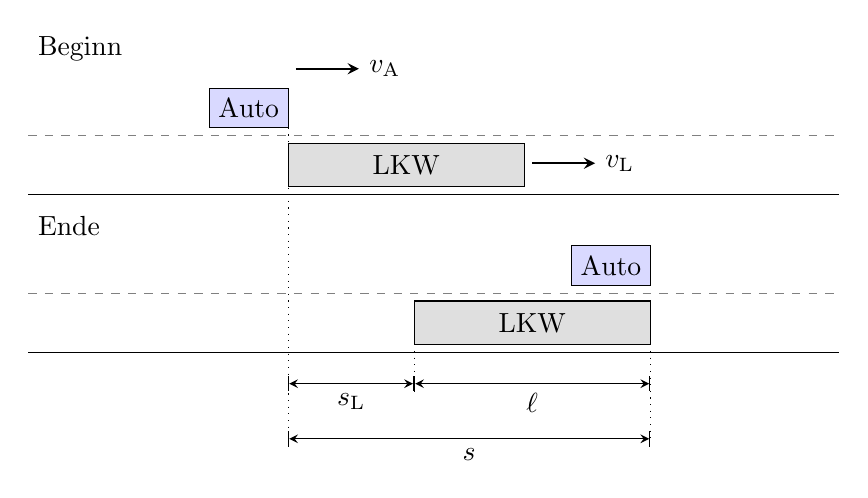
\begin{tikzpicture}[>=stealth]
 \draw (-0.3,2) -- (10,2);
 \draw[dashed, gray] (-0.3,2.75) -- (10,2.75);
 \node[anchor=west] at (-0.3,3.85) {Beginn};
 \draw[fill=gray!25] (3,2.1) rectangle (6,2.65) node[midway] {LKW};
 \draw[fill=blue!15] (2,2.85) rectangle (3,3.35) node[midway] {Auto};
 \draw[->, thick] (3.1,3.6) -- (3.9,3.6) node[right] {$v_\mathrm{A}$};
 \draw[->, thick] (6.1,2.4) -- (6.9,2.4) node[right] {$v_\mathrm{L}$};
 \draw (-0.3,0) -- (10,0);
 \draw[dashed, gray] (-0.3,0.75) -- (10,0.75);
 \node[anchor=west] at (-0.3,1.6) {Ende};
 \draw[fill=gray!25] (4.6,0.1) rectangle (7.6,0.65) node[midway] {LKW};
 \draw[fill=blue!15] (6.6,0.85) rectangle (7.6,1.35) node[midway] {Auto};
 \draw[dotted] (3,2.85) -- (3,-1.1);
 \draw[dotted] (4.6,0.1) -- (4.6,-0.5);
 \draw[dotted] (7.6,0.1) -- (7.6,-1.1);
 \draw[|<->|] (3,-0.4) -- (4.6,-0.4) node[midway, below] {$s_\mathrm{L}$};
 \draw[|<->|] (4.6,-0.4) -- (7.6,-0.4) node[midway, below] {$\ell$};
 \draw[|<->|] (3,-1.1) -- (7.6,-1.1) node[midway, below] {$s$};
\end{tikzpicture}
\end{center}

Die Länge des Autos und die Sicherheitsabstände sind vernachlässigt: Das Überholen beginnt, wenn die Spitze des Autos auf der Höhe des Lastwagenhecks ist, und endet, wenn sie die Spitze des Lastwagens erreicht. Das Auto fährt dabei die Strecke $s = s_\mathrm{L}+\ell$, also gegenüber dem Lastwagen die Strecke $\ell$, mit der Relativgeschwindigkeit $v_\mathrm{A}-v_\mathrm{L}$. Das dauert
\begin{align}
 t &= \tUF = \frac{\lL}{\vA-\vL} = \tU
\end{align}
In dieser Zeit legt das Auto den Überholweg
\begin{align}
 s &= v_\mathrm{A}\,t = \sUF \\
   &= \frac{\vA\cdot\lL}{\vA-\vL} = \sU \approx \result{\sUP{0}{2}}
\end{align}
zurück.
